\section{Overview}
\mikkel{WORKWORK: Merge this description with the architecture intro.
All subsections should be subsections and overview must die.}
\mikkel{WORKWORK: All macro component should \textbf{not} list their layers and then list then again.}
A system architecture is introduced to ease maintenance and ensure scalability.
The architecture consists of four macro components and a database, as can be seen in \Cref{fig:architecture}. The macro components are: Shared, Location Service, Model Agent, and Web Service.

\begin{figure}
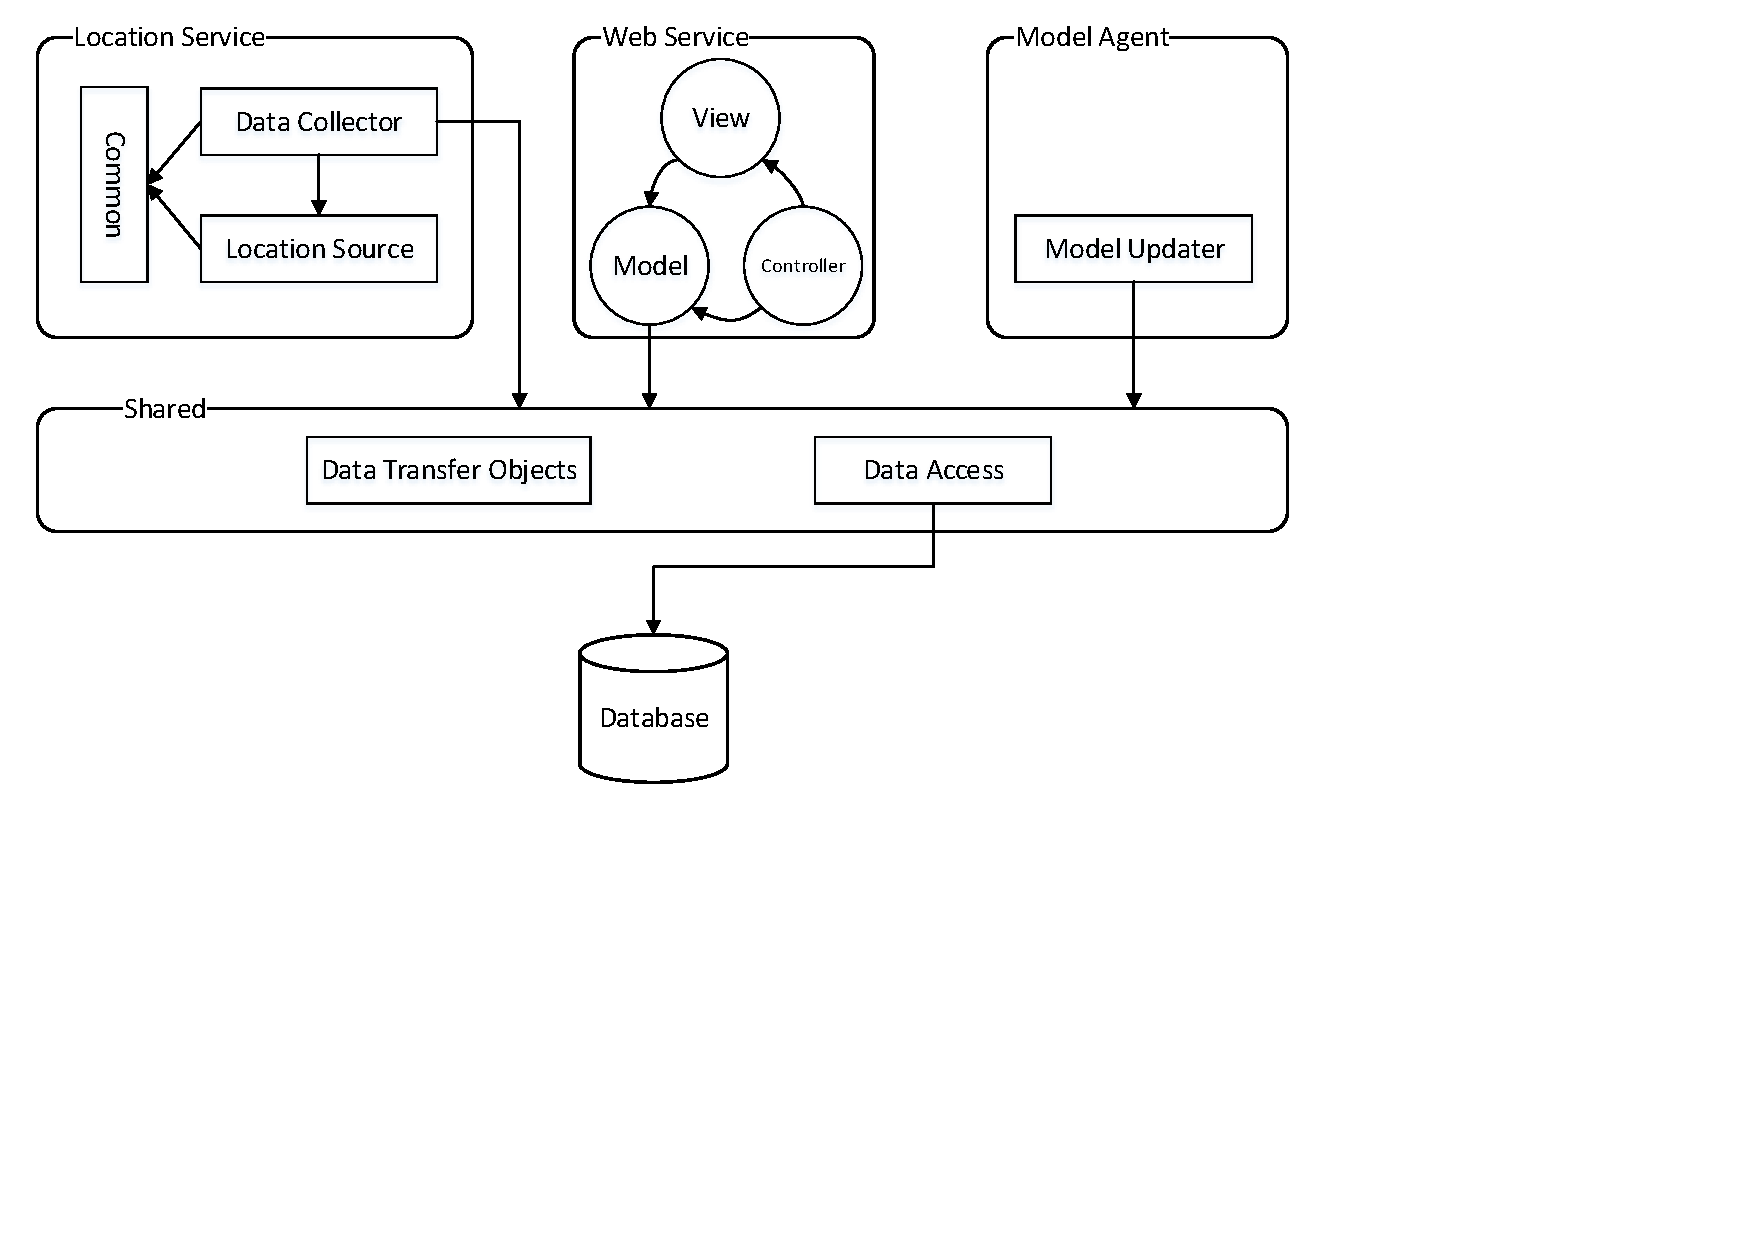
\includegraphics[width=\textwidth, trim={2cm 1cm 6cm 0}]{systemArchitecture.pdf}
\caption{The architecture of the system}
\label{fig:architecture}
\end{figure}

\subsection{Database} The database used is a MySQL database, and is where all our data is stored.
The design of the database can be found in \Cref{database_design}.
\mikkel{WORKWORK: Jeg synes vi mangler lidt argumentation for hvorfor designet ikke er inkluderet i rapporten.}

\subsection{Shared}
The task of the macro component shared is to provide extended capabilities to all other macro components.

\paragraph{The Data Access layer} All SQL statements and communication with the database are encapsulated here providing the upper layers a communication protocol to the database.
Additionally this layer provides an abstraction of the actual communication with the database as well as an abstraction of the database design.

\paragraph{The Data Transfer Object layer} contains all the shared data types and their attributes, making it possible for all the macro components to treat the data uniformly.
The types within this layer provides methods for retrieving data from the database and converting it into elements of the types in the Data Transfer Object layer.
\mikkel{Jeg synes vi mangler en beskrivelse af hvorfor der er forbindelse fra de tre øverste komponenter til Data Access. Men jeg kan ikke lige komme på en.}

\subsection{Location Service} 
The location service component processes and stores location data directly from a data source. 
The \texttt{Location Service} consists of a \texttt{Location Source} which provides data points to the \texttt{Data Collector}.
\mikkel{Jeg forestiller mig spørgsmål som ''What is The \texttt{Location Service} and a \texttt{Location Source}?''}

\paragraph{The Location Source layer} fetches data from the data source and then adapts it to the appropriate data type in the Common layer.
\stefan{cast? transform måske?}
It is structured so that the Location Source layer can easily be replaced with another source of data.

\paragraph{The Data Collector layer} gathers the data from the \texttt{Location Source} layer and processes it. 
The data is then stored through the \texttt{Data Access} layer.

\subsection{Model Agent}
\texttt{Model Agent}\footnote{An agent is defined as a program that invoke a given task, when a condition is satisfied, then returning to a sleeping state, until the condition is satisfied again.\cite{definitionagent}} is the macro component containing the \texttt{Model Updater} layer.
The macro component's task is to generate and update the model in the system. 

\paragraph{The Model Updater layer} handles the generation of the models.
The generation of the model works as follows:
Clusters are created based on the GPS data in the database \Cref{clustering:DBSCAN}.
The convex hull of the clusters is determined and saved as the hotspots of the model.
Markov chains are now created with these clusters as states \Cref{markov:create_model}.
\mikael{Tilføj noget om truncate}
\mikael{Fix referencer}

\subsection{Web Service}\label{arch:webservice}
Web Service is the macro component containing a Model, View, and Controller.
The task of the macro component is to provide a web service, in order for users to interact with the system.
The model, view, and controller of the web service were introduced in \Cref{??}.
\mikael{Her mangler reference til når MVC er blevet flyttet.}
